\chapter{Results}
\label{chapter_4}

\section{Experimental Setup}

\subsection{Dataset}

%%%
\subsection{Image Quality Assessment}

Denoising noise helps in eliminating noise from images, but may also create image distortion. Due to this, it is important to evaluate quality of denoised image in order to assess performance of a noise reduction method. The measures used to evaluate image quality in this internship include Mean Square Error (MSE) and Peak Signal to Noise Ratio (PSNR).

\textbf{Mean Square Error (MSE)}: Having the original image $f$ of the size $m \times n$ and its denoised image $f'$ of the same size, the mean square error is defined as follows:

%%%
\begin{equation}
    MSE = \frac{1}{mn}{\sum_{i=1}^{m}\sum_{j=1}^{n}(f'_{ij}-f_{ij})^2} 
\end{equation}

MSE is determined as the mean of square of the difference between the original image and its denoised image. MSE presents the quality of denoised image in the sense that the smaller MSE is the better quality the denoised image has. The ideal case is when MSE is equal to zero. It means that the noise is completely removed from the image.

%%%
\textbf{Peak Signal to Noise Ratio (PSNR)}: Having the MSE of the original image $f$ of the size $mxn$ and its denoised image $f'$ of the same size, the peak signal to noise ratio measure is determined as follows:

%%%
\begin{equation}
    PSNR = 10 \log_{10}\frac{R^2}{MSE}
\end{equation}

where $R$ is the maximum value of pixel intensity. For example, if the input image has an 8-bit unsigned integer data type, then R is equal to 255. The value of $PSNR$ presents for the quality of image. In other words, the higher the value of $PSNR$ is, the better quality the image has.

\textbf{Dataset}: The experiments are performed using a total of 20 photos in the ICTLab's SWARMS project dataset. Each photo is artifically noise-added with Gaussian noise. As previously described, this dataset is composed of 800 photos, collected by USTH bachelor students. These images are categorized into 4 groups: Construction site, Rubbish, Pagoda and Pond, each containing 200 photos. Figure~\ref{fig:example} shows examples of the four photo classes.


\begin{figure}[tb]
\begin{center}
	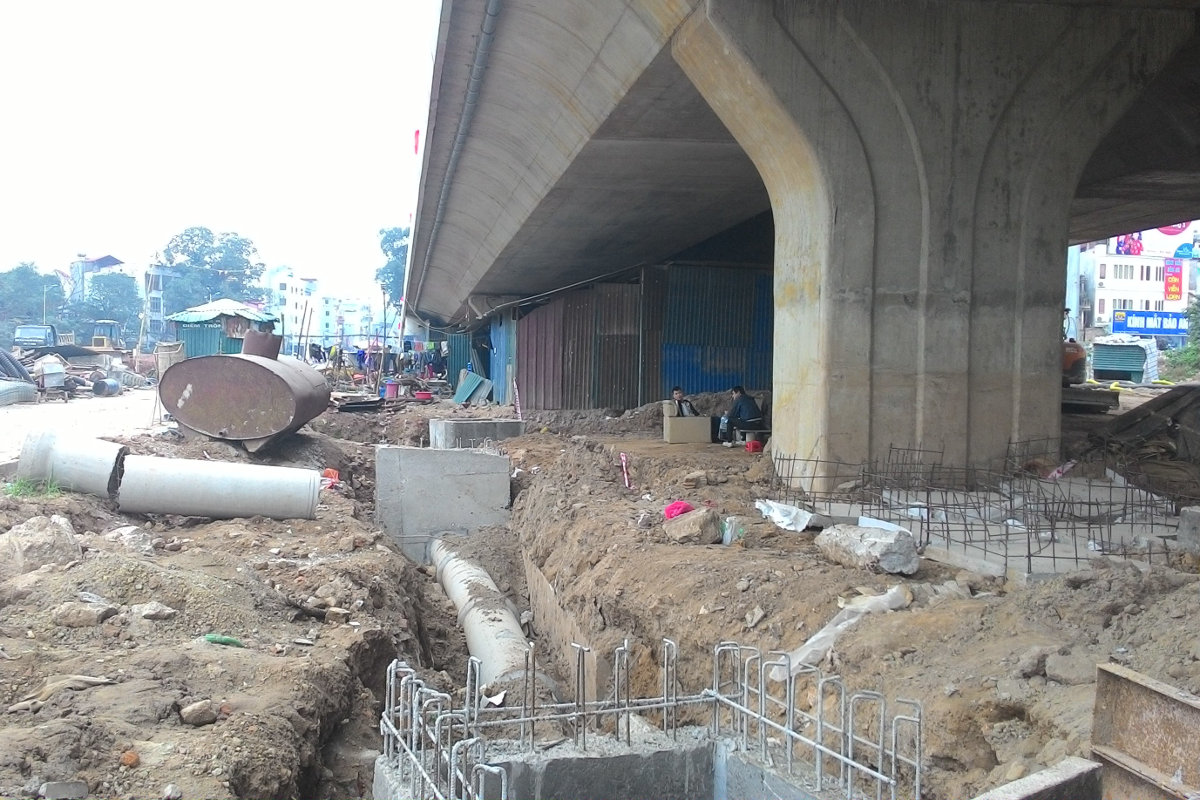
\includegraphics[width=0.24\columnwidth]{images/example-construction.jpg}
	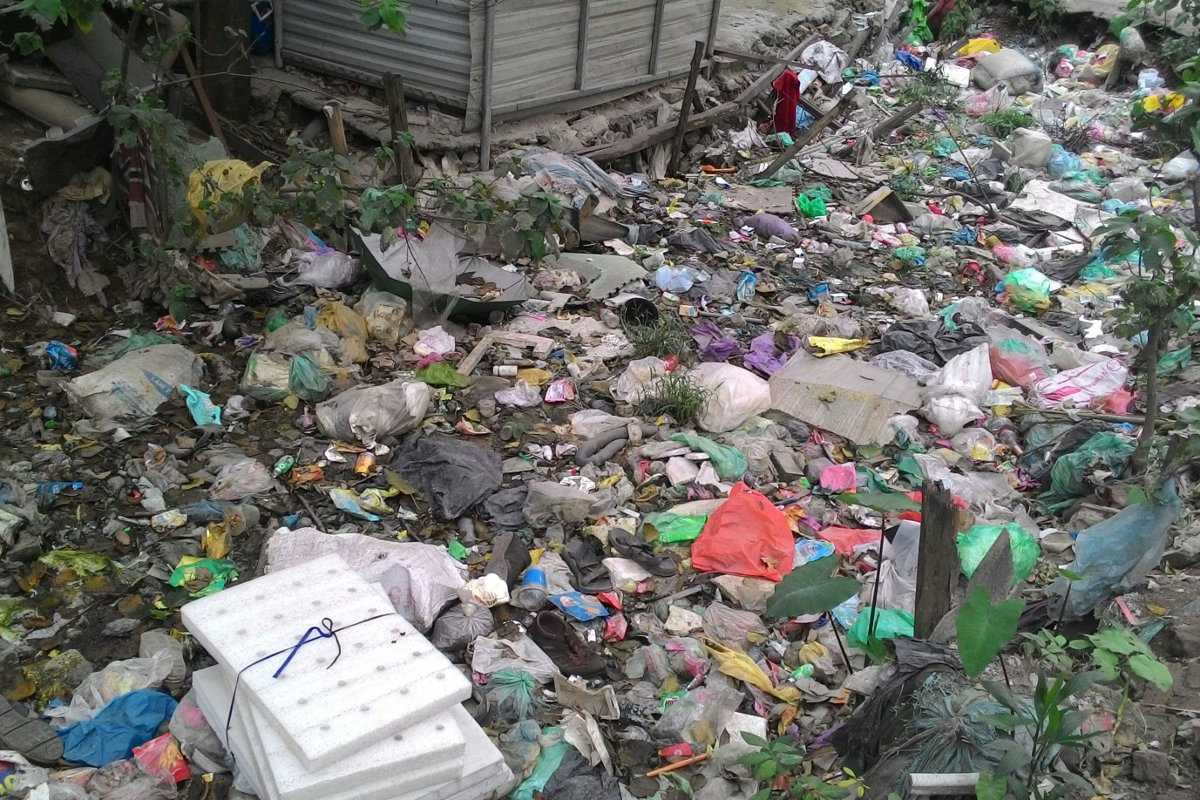
\includegraphics[width=0.24\columnwidth]{images/example-rubbish.jpg}
	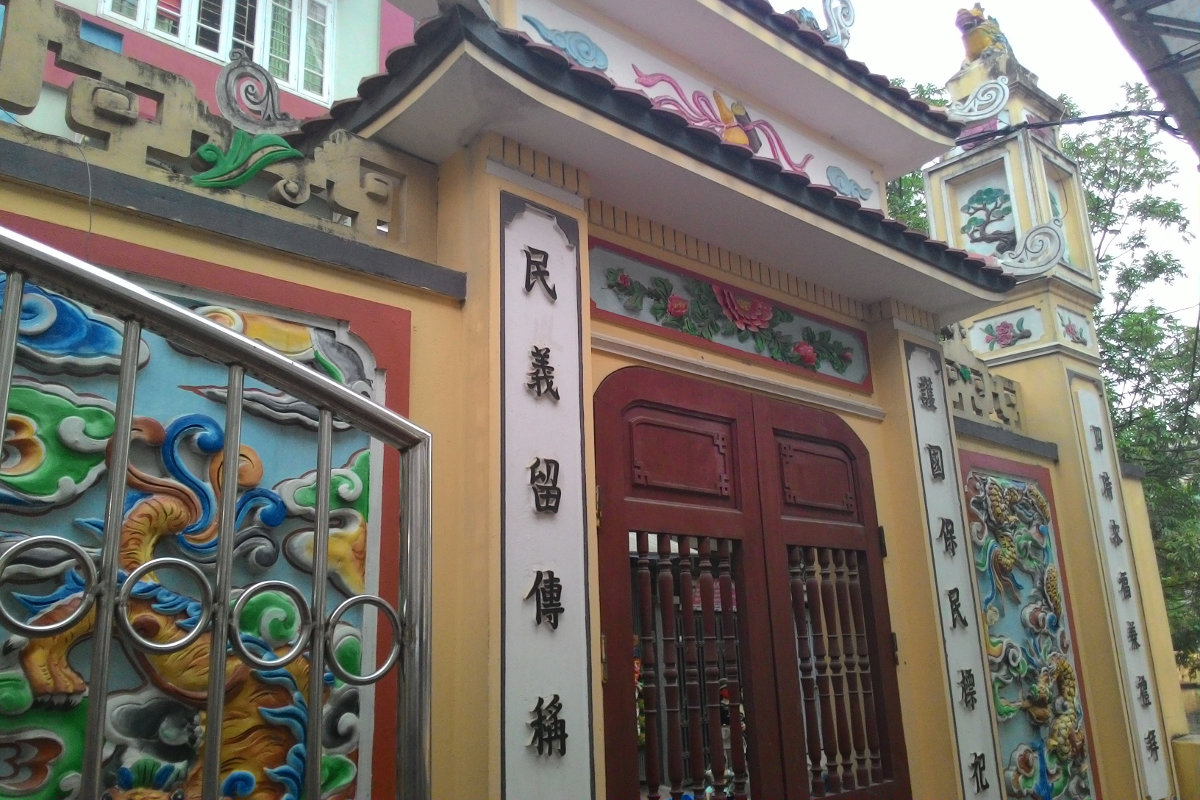
\includegraphics[width=0.24\columnwidth]{images/example-pagoda.jpg}
	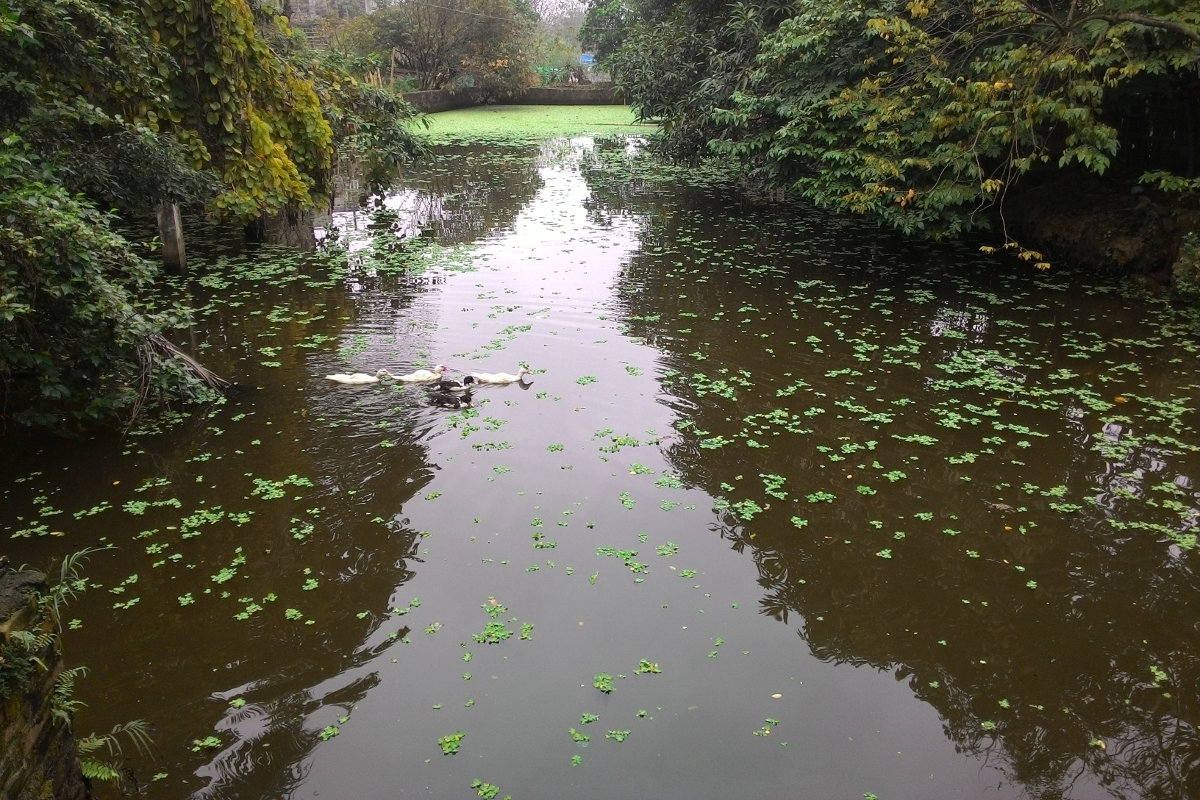
\includegraphics[width=0.24\columnwidth]{images/example-pond.jpg}
	\caption{Example of 4 photo classes. From left to right: Construction site, Rubbish, Pagoda, Pond}	
	
\end{center}
\end{figure}
%%%%
\section{Results and Discussion}

This section shows evaluation result of each described denoising method against 5 randomly chosen photos of each class. Expected results are answers to these questions:

\begin{itemize}
	\item Are the denoising methods effective? (i.e. can they reduce noise?)
	\item What is the best method for denoising SWARMS photos?
\end{itemize}

The next part of this section will present evaluation result for each photo category.

\newpage

\textbf{Construction Sites}

Figure~\ref{fig:construction} shows the images being used for the experiments in the first class. This class usually contains similar color tone and noise throughout the images.

\begin{figure}[h]
	\centering
	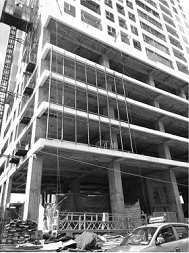
\includegraphics[width=0.18\columnwidth]{images/construction1.jpg}
	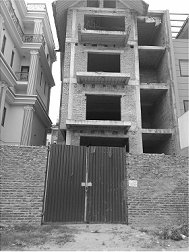
\includegraphics[width=0.18\columnwidth]{images/construction2.jpg}
	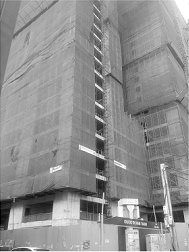
\includegraphics[width=0.18\columnwidth]{images/construction3.jpg}
	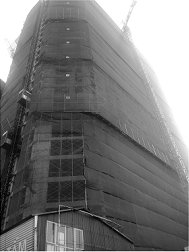
\includegraphics[width=0.18\columnwidth]{images/construction4.jpg}
	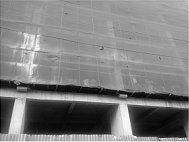
\includegraphics[width=0.18\columnwidth]{images/construction5.jpg}
	\caption{Evaluated construction site photos. From left to right: construction1, construction2, construction3, construction4, construction5}
	\label{fig:construction}
\end{figure}

\captionof{table}{Evaluated metrics for construction site photos}
\begin{center}
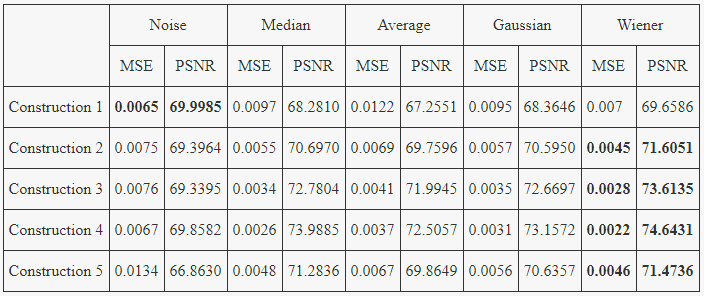
\includegraphics[width=15cm,height=7cm]{images/Construction.png}
\label{tab:construction}
\end{center}

\newpage

\textbf{Rubbish}

Figure~\ref{fig:rubbish} shows the images being used for the experiments in the second class. This class shows a large diversity of colors due to existence of different small objects in the photo.

\begin{figure}[h]
	\centering
	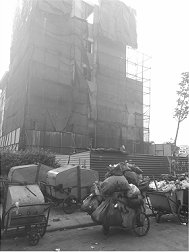
\includegraphics[width=0.18\columnwidth]{images/rubbish1.jpg}
	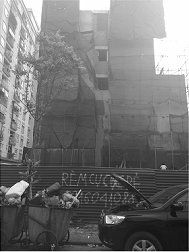
\includegraphics[width=0.18\columnwidth]{images/rubbish2.jpg}
	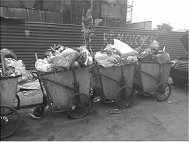
\includegraphics[width=0.18\columnwidth]{images/rubbish3.jpg}
	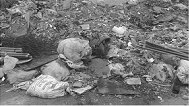
\includegraphics[width=0.18\columnwidth]{images/rubbish4.jpg}
	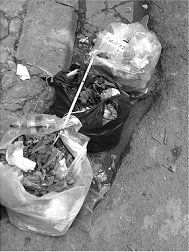
\includegraphics[width=0.18\columnwidth]{images/rubbish5.jpg}
	\caption{Evaluated rubbish photos. From left to right: rubbish1, rubbish2, rubbish3, rubbish4, rubbish5}
	\label{fig:rubbish}
\end{figure}

\captionof{table}{Evaluated metrics for rubbish photos}
\begin{center}
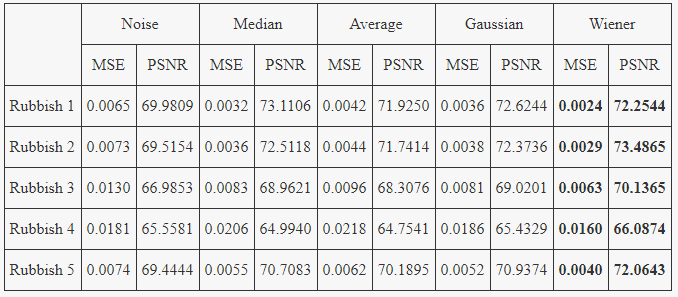
\includegraphics[width=15cm]{images/Rubish.png}
\label{tab:rubbish}
\end{center}

\newpage

\textbf{Pagoda}

Figure~\ref{fig:pagoda} shows the images being used for the experiments in the third class. This class show close color tone and noise for the images.

\begin{figure}[h]
	\centering
	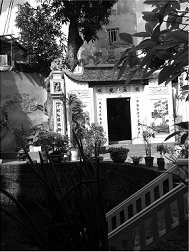
\includegraphics[width=0.18\columnwidth]{images/pagoda1.jpg}
	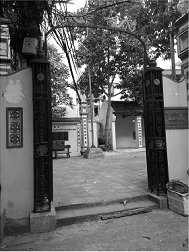
\includegraphics[width=0.18\columnwidth]{images/pagoda2.jpg}
	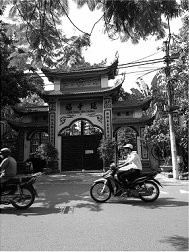
\includegraphics[width=0.18\columnwidth]{images/pagoda3.jpg}
	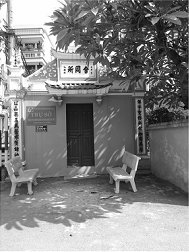
\includegraphics[width=0.18\columnwidth]{images/pagoda4.jpg}
	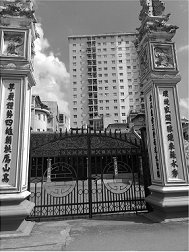
\includegraphics[width=0.18\columnwidth]{images/pagoda5.jpg}
	\caption{Evaluated pagoda photos. From left to right: pagoda1, pagoda2, pagoda3, pagoda4, pagoda5}
	\label{fig:pagoda}
\end{figure}


\captionof{table}{Evaluated metrics for pagoda photos}
\begin{center}
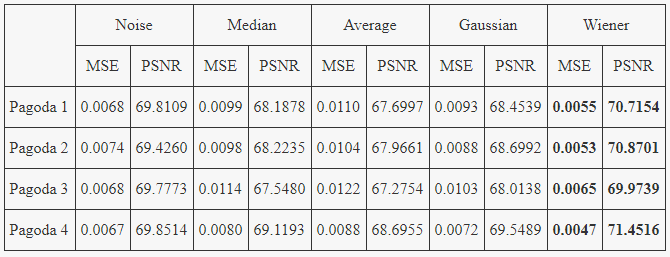
\includegraphics[width=15cm]{images/Pagoda.png}
\label{tab:pagoda}
\end{center}

\newpage

\textbf{Pond}

Figure~\ref{fig:pond} shows the images being used for the experiments in the third class. A lot of similarity in pixel intensities and very little diversion of noise are showed in this class.

\begin{figure}[h]
	\centering
	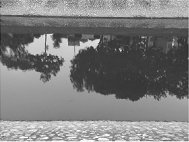
\includegraphics[width=0.18\columnwidth]{images/pond1.jpg}
	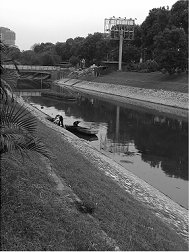
\includegraphics[width=0.18\columnwidth]{images/pond2.jpg}
	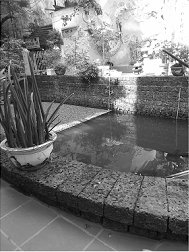
\includegraphics[width=0.18\columnwidth]{images/pond3.jpg}
	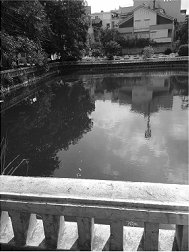
\includegraphics[width=0.18\columnwidth]{images/pond4.jpg}
	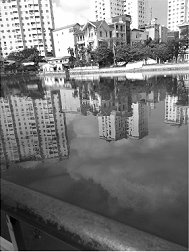
\includegraphics[width=0.18\columnwidth]{images/pond5.jpg}
	\caption{Evaluated pond photos. From left to right: pond1, pond2, pond3, pond4, pond5}
	\label{fig:pond}
\end{figure}


\captionof{table}{Evaluated metrics for pond photos}
\begin{center}
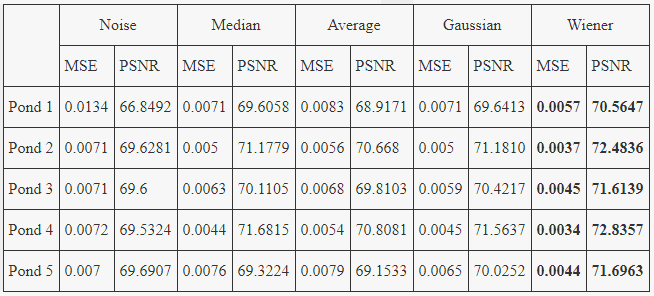
\includegraphics[width=15cm]{images/Pond.png}
\label{tab:pond}
\end{center}

\newpage

\setlength{\parskip}{0.5em}
\setlength\parindent{24pt}

\textbf{Discussion}

Tables~\ref{tab:construction}, \ref{tab:rubbish}, \ref{tab:pagoda} and \ref{tab:pond} show that in most cases of all categories, denoised images achieve smaller MSE and greater PSNR than the noisy image. This result indicates that all of the studied methods, namely Median filter, Average filter, Gaussian filter and Wiener filter, can reduce amount of noise in SWARMS dataset. These methods are therefore suitable for improving image quality for captured images.

To answer the second question from previous section, ``What is the best method for denoising SWARMS photos?'', it can be seen from all result tables that Weiner filter generally achieves best MSE and PSNR values, with one exception in rubbish2 photo. This accomplishment of Weiner filter can be explained as a result of its initial aim to minimize mean square error. However, this algorithm is performance-costly and (in average) takes 3.9 times longer than Average filter, 5.6 times longer than Gaussian filter and 1.3 times longer than Median filter.

Table~\ref{tab:runtime} presents this runtime result for one photo as delegation for each class in the dataset.

\captionof{table}{Method runtimes (in milliseconds)}
\begin{center}
	\begin{tabular}{| l | l | l | l | l |}
		\hline
		Photo 			& Median 	& Average 	& Gaussian 	& Weiner 	\\ \hline
		construction1	& 9.762		& 3.038		& 2.161		& 15.524	\\ \hline
		rubbish1		& 9.145		& 3.187		& 2.158		& 11.795	\\ \hline
		pagoda1			& 8.909		& 2.998		& 2.170		& 12.372	\\ \hline
		pond1			& 7.543		& 2.68		& 1.826		& 7.329		\\ \hline
	\end{tabular}
	\label{tab:runtime}
\end{center}